\documentclass[12pt]{article}
\usepackage{amsmath}
\usepackage{hyperref}
 \usepackage{graphicx}
 \usepackage{float}
 \usepackage{subcaption}
 \usepackage{listings}

\title{Analysis of Convolution with Original, Modified, and Shifted Kernels on Inverse Trigonometric Functions}
\author{Arnav Yadnopavit}
\date{\today}

\begin{document}

\maketitle


\section*{1. Original Kernel}
The \textbf{original symmetric kernel} $h(t)$ defined as:
    \[
    h(t) = 
    \begin{cases}
        1, & \text{for } -T \leq t \leq T \\
        0, & \text{otherwise}
    \end{cases}
    \]
The symmetric kernel includes both past and future values around time $t$. When this kernel is convolved with the inverse trigonometric functions:
\begin{itemize}
    \item The result is a \textbf{smoothed} version of the original signal.
    \item The kernel acts like a moving average centered at each point.
    \item For $\arcsin(t)$ and $\arccos(t)$, the undefined regions outside $[-1,1]$ are managed using $\texttt{np.clip}$, leading to saturation outside that interval.
    \item The convolution retains the central trend and symmetry of the original signal.
\end{itemize}
\begin{figure}[H]
    \centering
    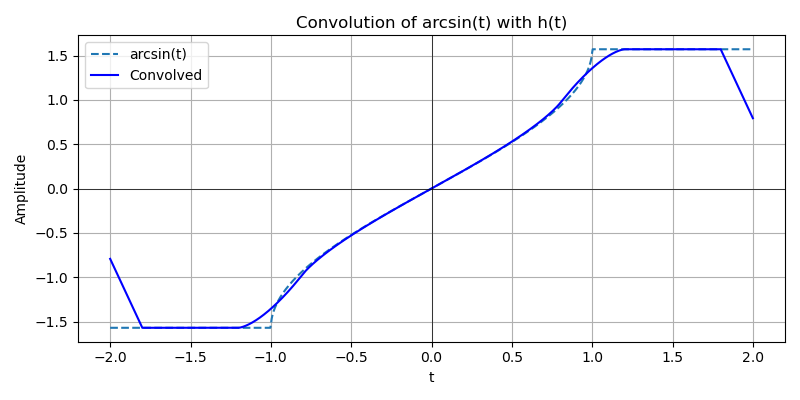
\includegraphics[width=0.7\textwidth]{figs/org1.png}
\end{figure}
\begin{figure}[H]
    \centering
    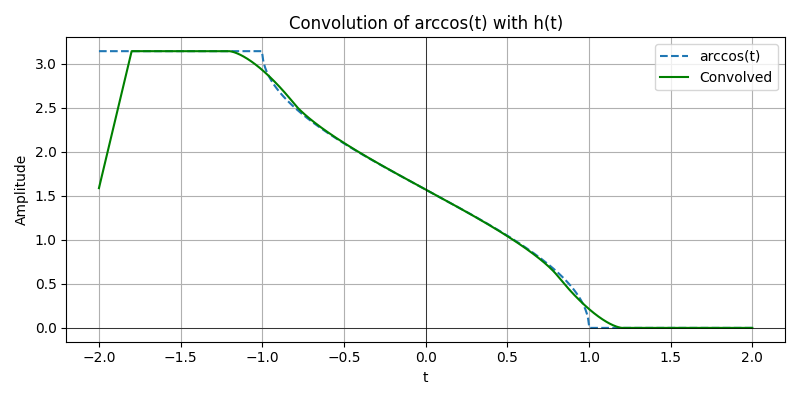
\includegraphics[width=0.7\textwidth]{figs/org2.png}
\end{figure}
\begin{figure}[H]
    \centering
    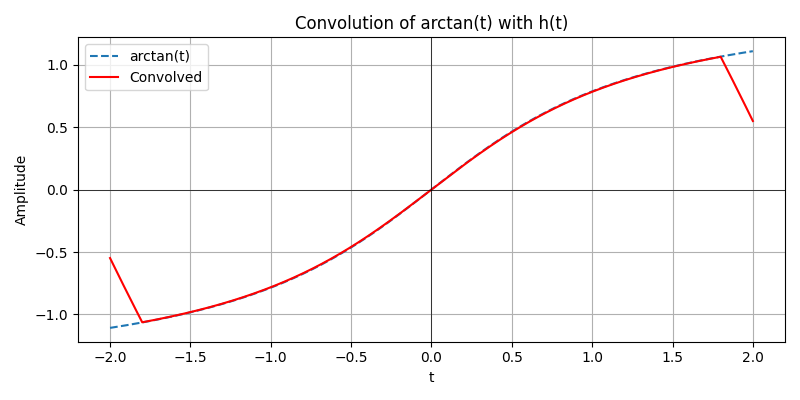
\includegraphics[width=0.7\textwidth]{figs/org3.png}
\end{figure}
\section*{2. Modified One-Sided Kernel}
The \textbf{modified one-sided kernel} that only considers $t > 0$:
    \[
    h(t) = 
    \begin{cases}
        1, & \text{for } 0 < t \leq T \\
        0, & \text{otherwise}
    \end{cases}
    \]
The one-sided kernel (nonzero only for $t > 0$) introduces an inherent \textbf{asymmetry} into the convolution:
\begin{itemize}
    \item It models a \textbf{causal} system—one that responds only to the present and past.
    \item The output becomes more biased toward \textbf{past values}, creating a smoothing effect that \textbf{lags behind} the original function.
    \item For $\arcsin(t)$ and $\arccos(t)$, the convolution output shows a shift toward the left and becomes less symmetric.
    \item For $\arctan(t)$, the effect is more subtle but still causes a smoothing that trails the input.
\end{itemize}
\begin{figure}[H]
    \centering
    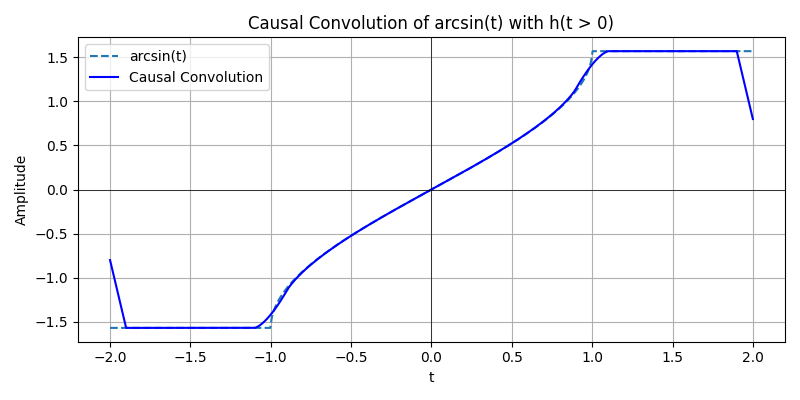
\includegraphics[width=0.7\textwidth]{figs/mod1.png}
\end{figure}
\begin{figure}[H]
    \centering
    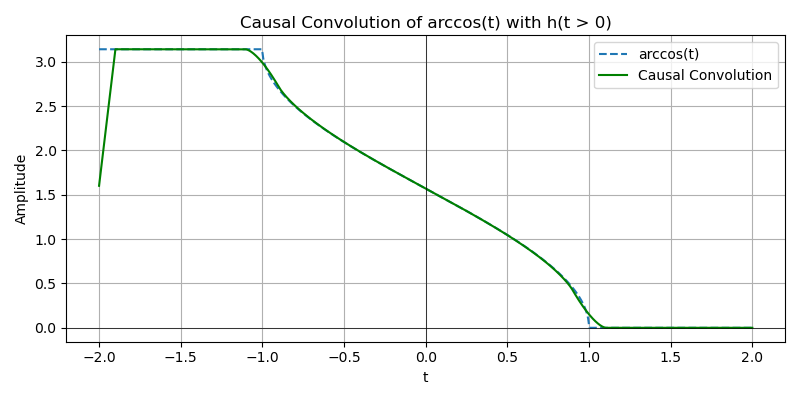
\includegraphics[width=0.7\textwidth]{figs/mod2.png}
\end{figure}
\begin{figure}[H]
    \centering
    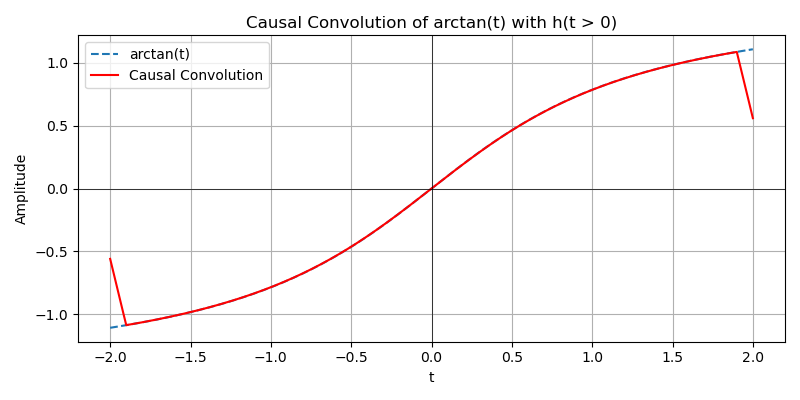
\includegraphics[width=0.7\textwidth]{figs/mod3.png}
\end{figure}
\section*{3. Shifted Kernel}
Convolving with $h(t - \tau_0)$ introduces a time delay of $\tau_0$ into the output:
\begin{itemize}
    \item The \textbf{shape} of the convolution result remains essentially unchanged.
    \item The entire output is \textbf{delayed} by $\tau_0$, modeling systems with fixed time delay (e.g., transmission delays).
    \item This shift preserves symmetry and smoothness, unlike the one-sided kernel.
    \item Such modeling is useful in time-delayed systems in control and signal transmission.
\end{itemize}
\begin{figure}[H]
    \centering
    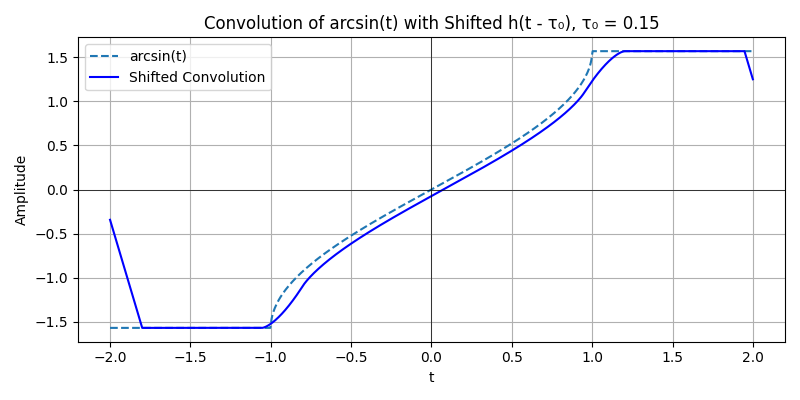
\includegraphics[width=0.7\textwidth]{figs/shift1.png}
\end{figure}
\begin{figure}[H]
    \centering
    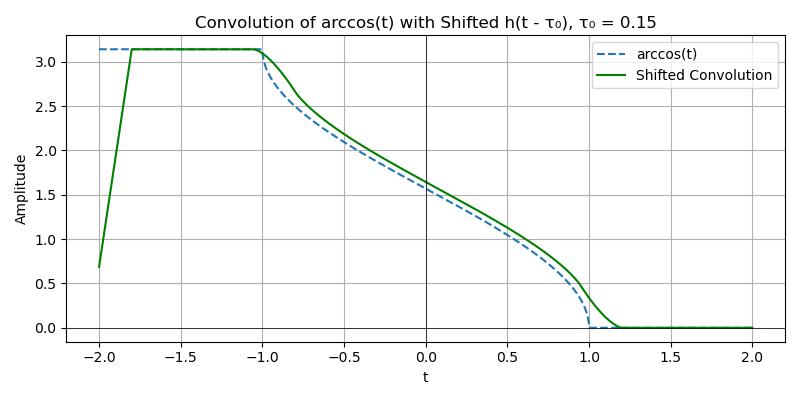
\includegraphics[width=0.7\textwidth]{figs/shift2.png}
\end{figure}
\begin{figure}[H]
    \centering
    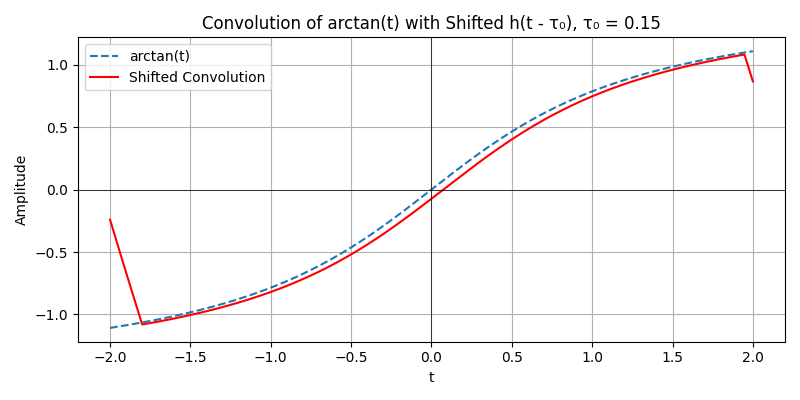
\includegraphics[width=0.7\textwidth]{figs/shift3.png}
\end{figure}
\section*{Conclusion}
Each type of kernel plays a different role:
\begin{itemize}
    \item The \textbf{original kernel} performs symmetric smoothing.
    \item The \textbf{modified kernel} introduces causality and asymmetry.
    \item The \textbf{shifted kernel} adds a pure delay without distorting the function shape.
\end{itemize}

\end{document}

